\documentclass[conference]{IEEEtran}

\usepackage{amsmath, amsthm, amssymb, dsfont, accents}

\usepackage{tikz}
\usepackage{hyperref, booktabs}
\usepackage{biblatex}

\usetikzlibrary{calc, automata}

\addbibresource{2_references.bib}

\pdfinfo{
   /Author (Homer Simpson)
   /Title  (Robots: Our new overlords)
   /CreationDate (D:20101201120000)
   /Subject (Robots)
   /Keywords (Robots;Overlords)
}

% MDPs
\newcommand{\MDP}{\mathbb{M}}

\newcommand{\X}{\mathbb{X}}
\newcommand{\U}{\mathbb{U}}
\newcommand{\init}{\rho}
\newcommand{\tr}{T}

\newcommand{\pol}{\mu}

% LTL
\newcommand{\True}{\texttt{true}}
\newcommand{\False}{\texttt{false}}
\newcommand{\AP}{AP}

\newcommand{\ltluntil}{\mathcal{U}}
\newcommand{\ltlnext}{\bigcirc}

\newcommand{\alphabet}{{2^{\AP}}}
\newcommand{\word}{\boldsymbol{\pi}}
\newcommand{\letter}{\pi}
\newcommand{\lab}{L}

\newcommand{\FSA}{\mathcal{A}}

% Probability
\newcommand{\Prob}{\mathbf{P}}


% Value iteration
\newcommand{\bellman}{\mathcal{B}}


% Math
\DeclareMathOperator*{\argmin}{arg\,min}
\DeclareMathOperator*{\argmax}{arg\,max}
\newcommand{\ind}{\mathbf{1}}


\newtheorem{problem}{Problem}
\newtheorem{definition}{Definition}
\newtheorem{remark}{Remark}
\newtheorem{example}{Example}

\newcommand{\red}[1]{{\color{red} #1 }}

\begin{document}

\title{\huge Report 3 }

\author{PN et al}

\maketitle

\begin{abstract}
Motivated by autonomy in space, we study the difficult problem of planning under uncertainty and capacity constraints. By leveraging ideas from formal synthesis and belief-space roadmaps, we synthesize a reactive strategy that maximizes the probability of satisfying certain high-level objectives, while guaranteeing that a safety-critical specification is satisfied throughout the mission.  
\end{abstract}

\IEEEpeerreviewmaketitle

  
%%%%%%%%%%%%%%%%%%%%%%%%%%%%%%%%%%%%%%%%%%%%%%%%
%%%%%%%%%%%%%%%%%%%%%%%%%%%%%%%%%%%%%%%%%%%%%%%%

\section{Problem Setup}

\subsection{Dynamics}

The overall concrete state is $x = (x^r, x^c)$, where $x^r$ is the state of the rover and $x^c$ the state of the copter. There are control inputs $u^r$ and $u^c$ to the two systems. In addition, the environment model is represented with a (stationary but unknown) map state $m \in L^{n^m}$, where $L$ is a set of pre-defined labels.

\subsection{Copter Dynamics}

We assume that the copter state is $(x^c, p^c)$ where $p^c \in \{ 0,1 \}$ determines whether the copter is at the ground or airborne. When it is airborne it can move freely between regions at a bounded speed, but is constrained by its battery capacity $\lambda$ that limits its total movement throughout the mission. When the copter is airborne $\lambda$ decreases at a rate proportional to the distance traveled:
\begin{equation}
  \frac{\mathrm{d}}{\mathrm{d}t} \lambda(t) = \begin{cases}
    -1 & p^c = 1, \\
    0 & \text{otherwise}.
  \end{cases}
\end{equation}

\subsubsection{Belief Dynamics}

We assume that we can observe outputs $y = (y^r, y^c, y^m) = h(x^r, x^c, x^m, w^y)$ of the rover, copter, and map that may be corrupted by stochastic or bounded noise $w^y$. Based on these measurements, we maintain belief states $b(t) \in \mathbb{B}$ that are updated according to some deterministic filter $\tau : \mathbb{B} \times \mathbb{U} \times \mathbb{Y} \rightarrow T \mathbb{B}$:
\begin{equation}
  \dot b = \tau(b, u, y).
\end{equation} 
The overall augmented system thus becomes
\begin{equation}
\label{eq:belief}
\begin{aligned}
  & \dot x^r = f^r(x^r, u^r, w^r), \\
  & \dot x^c = f^c(x^c, u^c, w^c), \\
  & \dot b = \tau(b, u^c, u^r, h(x^r, x^c, m, w^y)),
\end{aligned}
\end{equation}
where $w^r$ $w^c$ and $w^y$ are aggregated noise entering the system at different locations. A control policy for the overall system is a (potentially hybrid) system with input $b$ and outputs $u^r$ and $u^c$. As a special case stochasticity can be removed from parts of the system and a perfect output map can be assumed, which reduces the belief state to the concrete state. 

When $\tau$ is a Kalman filter, the belief state is ($\hat x, P)$, where $\hat x$ is the current state estimate and $P$ represents the covariance of $x - \hat x$. In this case, the dynamics of $P$ are deterministic but the state estimate $\hat x$ is affected by the noise and is thus a stochastic process.


\subsection{Specification}

A crucial part of the safety specification is the following guarantee that the copter behaves in a safe way:
\begin{equation}
  \square (\lambda \geq 0) \land p^c \implies x^c \; \text{safe} \land p^c(T) = 0.
\end{equation}


\subsection{Problem Statement}

In this work we seek to synthesize reactive controllers in belief space in order to achieve two things: satisfaction of a safety-critical specification with very high probability, and maximization of the probability that a set of non-safety critical target specifications are satisfied. In particular, we consider a safety specification $\varphi_S$ and a set of target specifications $\{ \varphi_{T_i} \}_{i \in I}$ and seek to approximately solve the following problem:
\begin{equation}
\begin{aligned}
  \argmax_{\pol} & \quad  \sum_{i \in I} \mathbb{P} \left( \xi \models \varphi_{T_i} \right), \\ 
  \text{s.t.} &\quad   \mathbb{P} \left( \xi \models \varphi_S \right) \geq 1 - \delta.
\end{aligned}
\end{equation}


For certain infinite-horizon properties and types of stochastic noise, the probability of specification violation is 1 for any control policy \cite{Ehlers2016}. For this reason we consider satisfaction over a finite horizon $[0, T]$ by assuming that no further movement is possible for $t > T$.


\section{Demo}


This is a non-formal description of a potential demo scenario. The more theoretical guarantees we can have with respect to one of the above frameworks, the better!

Equipment:
\begin{itemize}
  \item Quadrotor,
  \item Rover,
  \item Monitor displaying current belief for environment (safety probability for each region, variance).
\end{itemize}


\paragraph{Environment and exploration:} Collection of regions $\{ M_i \}$ such that $M_i \cap M_j = \emptyset$, and $\cup_i M_i$ is the whole work space. Each region $i$ has a binary label $l^i$ indicating that it is safe ($l^i = 1$) or unsafe ($l^i=0)$. Initially, there is a prior belief over labels that has high confidence only for regions close to the starting point. The quadrotor can estimate the label of regions it flies over with a confidence level that is inversely proportional to distance. For instance, the quadrotor can be assumed to receive a measurement of $l^i$ each second, drawn from $\mathcal N(l^i, \gamma(\| x^i - \mathbf{r}^c \|_2) )$, where $x^i \in \mathbb{R}^2$ is the center of region $i$ and $\gamma$ is a class $\mathcal K_\infty$-function.


\paragraph{Specifications:}

\begin{itemize}
  \item Let $A$ and $B$ be sets of regions. The rover should visit at least one $A$-region and at least one $B$-region.
  \item The rover can not visit unsafe regions.
  \item Quadrotor can only land in safe regions.
\end{itemize}


\paragraph{Practical details:} State estimation done via motion-capture for both quadrotor and rover.


\paragraph{What do we need to make this happen?}

\begin{itemize}
  \item Abstraction of quadrotor behavior providing an interface amenable to planning.
  \item Abstraction of rover behavior providing an interface amenable to planning.
  \item Planning to orchestrate rover and quadrotor motion.
  \begin{itemize}
    \item Simplest meaningful planning space: rover and copter spatial locations (2D + 3D), map belief space.
  \end{itemize}
  \item Quadrotor controller that can follow plan for take-off, flight, and landing.
  \item Rover controller that can follow plan.
\end{itemize}

\section{Toy Example}

\subsection{Toy example}

Consider a world with four regions $s_1, s_2, s_3, s_4$ and the following transitions:

\begin{center}
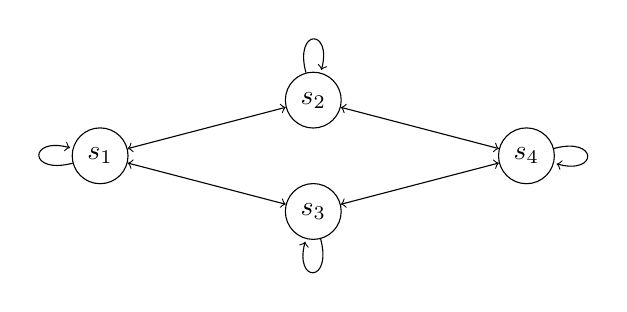
\begin{tikzpicture}
  \node[circle, draw] (s1) {$s_1$};
  \node[circle, draw, above right of=s1, xshift=2cm] (s2) {$s_2$};
  \node[circle, draw, below right of=s1, xshift=2cm] (s3) {$s_3$};
  \node[circle, draw, below right of=s2, xshift=2cm] (s4) {$s_4$};
  \draw[-latex, <->] (s1) -- (s2);
  \draw[-latex, <->] (s1) -- (s3);
  \draw[-latex, <->] (s2) -- (s4);
  \draw[-latex, <->] (s3) -- (s4);
  \path (s1) edge[loop left] (s1)
      (s2) edge[loop above] (s2)
      (s3) edge[loop below] (s3)
      (s4) edge[loop right] (s4);
\end{tikzpicture}
\end{center}

A copter and a rover can be controlled to move between these regions; the current region captured by states $\xi^c, \xi^r \in \{ s_1, s_2, s_3, s_4 \}$. Each region $s_i$ can be safe or unsafe, as captured by a binary unknown label $\bar l_i$. The label is estimated via a belief state $(\hat l_i, \hat \sigma^2_i)$. When the copter visits a state $s_i$ it receives a measurement $l_i$ drawn from $\mathcal N(\bar l_i, \sigma_i^2)$ and updates the estimate. This gives the belief dynamics
\begin{equation}
\begin{aligned}
(\hat l_i)^+ =
\begin{cases}
  \frac{\hat \sigma^2_i l_i + \sigma_i^2 \hat l_i}{\sigma_i^2 + \hat \sigma_i^2}, & \xi^c = s_i, \\
  \hat l_i, & \text{otherwise,}
\end{cases}
\quad (\hat \sigma_i^2)^+ = 
\begin{cases}
  \frac{\hat \sigma_i^2 \sigma_i^2}{\hat \sigma_i^2 + \sigma_i^2}, & \xi^c = s_i, \\
  \hat \sigma_i^2, & \text{otherwise,}
\end{cases}
\end{aligned}
\end{equation}
which is a nonlinear stochastic system. Let the specification be
\begin{equation}
  \lozenge (\xi^r = s_4) \land \bigwedge_{i=1}^4 \square \left[ (\xi^c = s_i) \implies (\hat l_i -3 \hat\sigma_i > 0) \right]
\end{equation}
and assume initial conditions
\begin{equation}
\begin{aligned}
  & \xi^c = \xi^r = s_1, & \\
  & \hat l_1 = \hat l_4 = 1, \quad   & \hat \sigma_1 = \hat \sigma_4 = 0, \\
  & \hat l_2 = \hat l_3 = 0.5, \quad & \hat \sigma_2 = \hat \sigma_3 = 0.5.
\end{aligned}
\end{equation}

\begin{itemize}
  \item A solution may not exist \\
  \item Could impose assumptions on $\bar l_2$ and $\bar l_3$ to ensure existence ($\bar l_2 + \bar l_3 \geq 1$) \\
  \item Without assumptions, can we find strategy that maximizes $\mathbb{P} \left[ x \models \phi \right]$?
\end{itemize}
Can we ``solve'' this with FIRM? Can create one FIRM object per state and consider cross space of 5 transition systems where state of copter is input to FIRM.

\end{document}
